\documentclass[11pt]{article}
\usepackage{amsfonts}
\usepackage{amsmath}
\usepackage[makeroom]{cancel}
\usepackage[top=.5in, bottom=1in, left=.5in, right=.5in]{geometry}
\fontsize{15}{2} 
\allowdisplaybreaks[1]
\usepackage{setspace}
\onehalfspacing
\usepackage{listings}
\usepackage{hyperref}
\usepackage{marvosym}
\usepackage{courier}
\usepackage{graphicx} % more modern
\usepackage{subfigure} 
\usepackage{caption}
\usepackage{listings}
\def\etal{{\textit{et~al.~}}}

\begin{document}

\vspace*{8cm}

\centerline{\sc \Large Machine Learning and Computational Statistics: Project Report}

\vspace{1cm}

\centerline{\sc \small Emily Denton (eld297)  \& Rahul Gopalkrishnan (rg2451)}
         
\clearpage 


\section{Introduction}


\section{Problem definition}

\subsection{Learning a word embedding space}

In order to learn an embedding of words into a vector space, we use the training code provided by Mikolov \etal in word2vec\cite{word2vec}. There are two different models, the Skip-Gram model and the Continuous Bag of words (CBOW) model. Both models consist of a projection layer followed by a softmax layer. They differ in the precise inputs and outputs used. The training data for both models consists of a sequence of words, $w_1, w_2, ..., w_N$. Let $M$ denote the size of the vocabulary (i.e. the number of distinct words in the entire training sequence). We described each of them in turn. 

\subsubsection{Skip Gram}
The Skip-Gram model takes a single word as input and aims to predict the surrounding words, where the order of the surrounding words matters. More specifically, we want to find the parameters $\theta$ which maximize the conditional log probability of the context of a given word:

\begin{align*}
	\sum_{n=1}^{N} [\sum_{-c \leq t \leq c; t \neq n} \log p(w_{n+c} | w_n; W)]
\end{align*}
where $c$ is the size of the context window being considered (in our experiments we set c = 6). 

The output probability is given by
\begin{align*}
p(w_{O} | w_{I}; W) = \frac{ \exp \big(\psi(w_O) \cdot \phi(w_I) \big)}{\sum_{j=1}^M \exp \big(\psi(w_j) \cdot \phi(w_I) \big)}
\end{align*}


where $\phi(w_i) = W^{\top}x_i$ is the vector representation of $w_i$ (letting $x_i$ denote the 1-hot input vector for with i) and $\psi(w_i)$ is the output representation for word $w_i$ (this can be thought of as the outgoing weights from the projection layer to the softmax unit corresponding to word $w_i$ . The parameters of the system are learned via gradient descent. After training, the final vector representations, $\phi(w_i) \forall i$, are computed from the matrix $W$.



\subsubsection{Continuous Bag of Words (CBOW)}
Unlike the skip gram model, the CBOW model makes a bag of words assumption by projecting all words in the context of a given word into the same position and, from that vector, trying to predict the word. The goal of learning is to find the parameters $W$ that maximize the conditional log probability of a word, given the surrounding words. 
\begin{align*}
	\sum_{n=1}^N \log p(w_n| u;\theta) \hspace{5mm} \text{ where } u = \sum_{-c \leq t \leq c; t \neq n} \phi(w_{n+c} )
\end{align*}


Ultimately, after training either the Skip-Gram or the CBOW model, the result is a $D$ dimensional embedding space for the words in the vocabulary. In all of our experiments we use $D = 300$. 

Google has published 3 million 300-dimensional word vectors trained with a Skip-Gram model on Google News data. We also trained our own CBOW and Skip-Gram models. One of our goals of this project was to explore the effect of training set size on the regularities present in the embedding space. Our models are trained on a sizable corpus, but this comes no where close to the kind of data Google has access to. In section \ref{results:analogy} we quantify how good the learned embedding spaces are for the Google vectors and our own models. 

\begin{figure}[h]
\centering
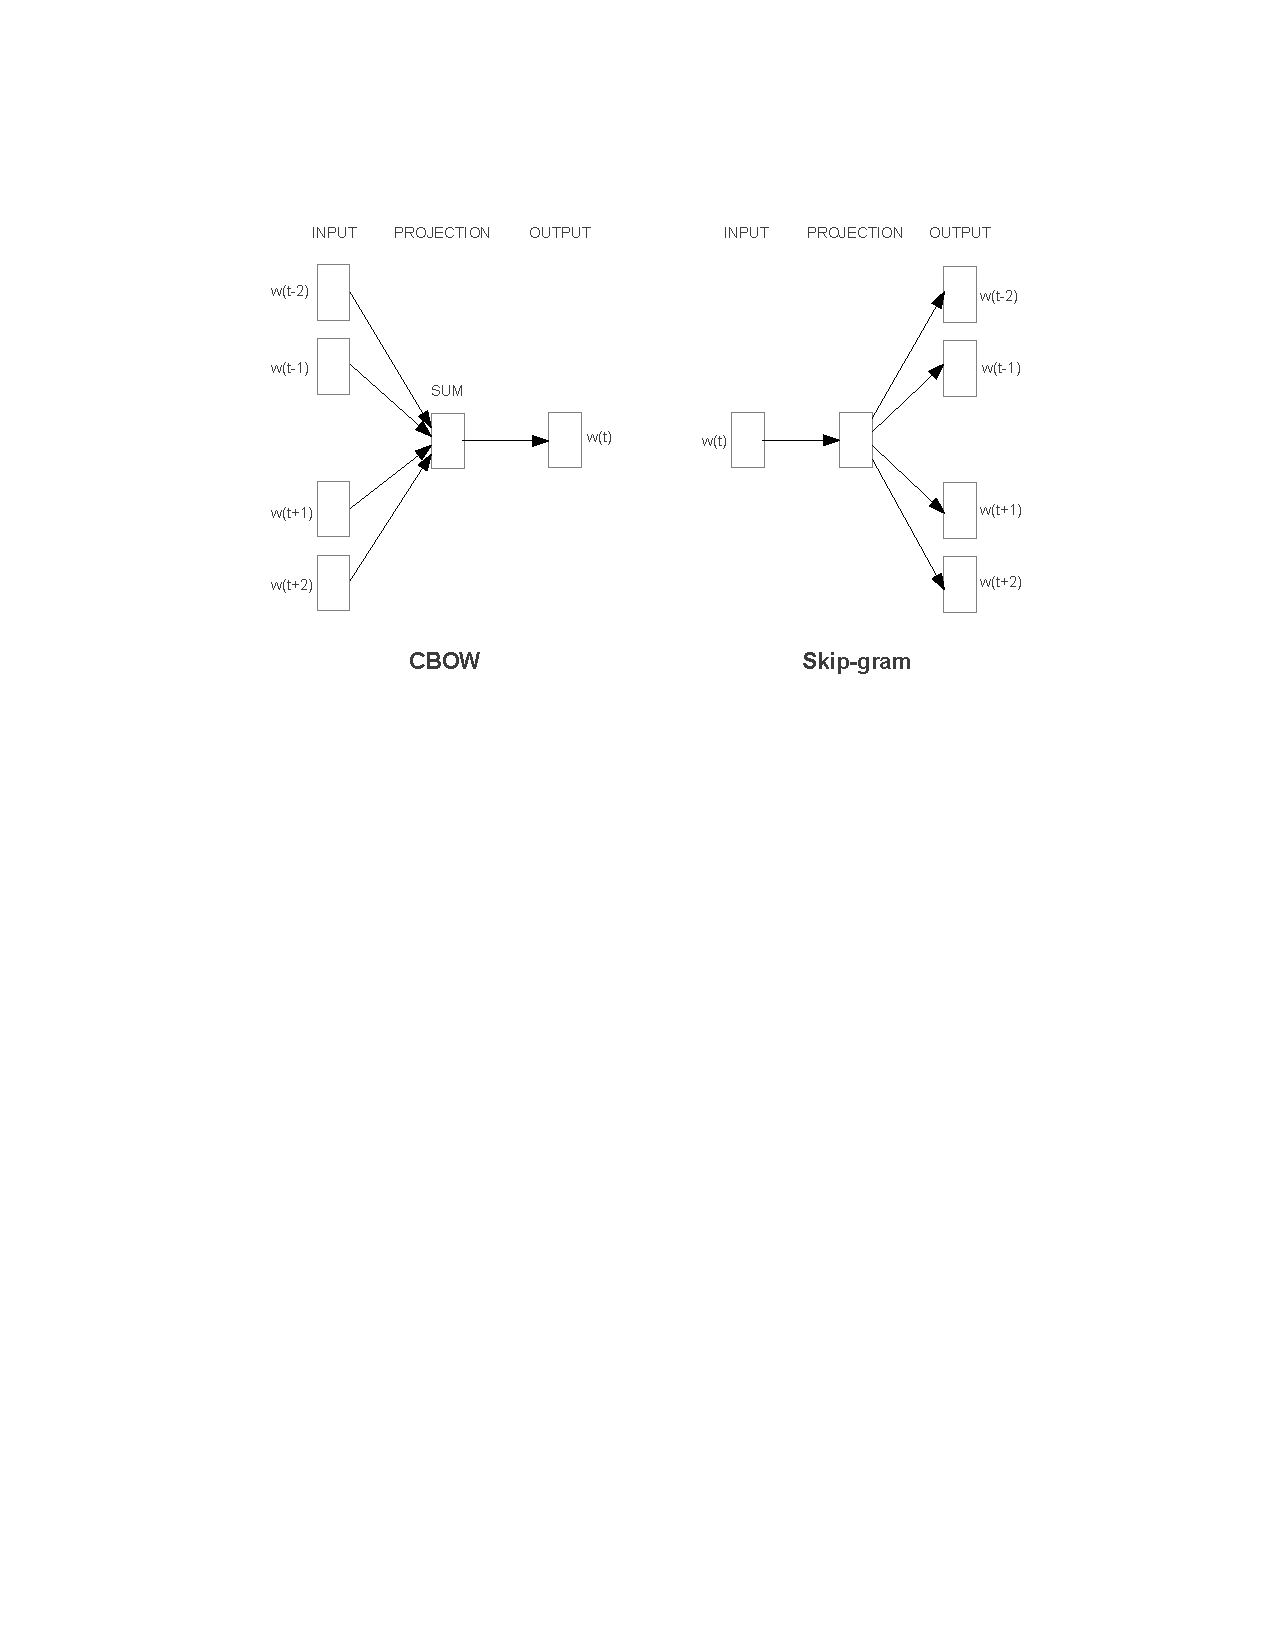
\includegraphics[width=\textwidth]{./images/model_images.pdf}
\caption{CBOW and Skip-Gram Models. Image adopted from \cite{mikolov1}}
\label{fig:top_k}
\end{figure}

\clearpage 


\subsection{Exploring properties of learned word embedding space}

There has been increased interest gathering around the embedding spaces that are learned via these simple log-linear models. Mikolov \etal. \cite{mikolov3} \cite{mikolov4} have shown that the embedding spaces exhibit interesting linear structure that can be exploited to solve a variety of language tasks. For example, they show that the word vectors can be used to solve analogical reasoning questions of the form "{\it King}" is to "{\it man}" as "{\it Queen}" is to "\_\_". They also show that embedding spaces for different languages have similar geometric structure and thus words can be translated from language A to language B by learning a simple linear transformation from the embedding space for language A to the embedding space for language B. 

Our second goal of this project was to explore the linear structure present in the embedding spaces. In section \ref{sec:results} we present a variety of results. We show different ways of visualizing the low dimensional structure of the embedding spaces. We show results on approximating different subsets of word vectors with low rank approximations. Finally, we show how to automatically discover analogical relations for a set of word vectors. 

The overarching goal of this work is to gain insight into the structure of the word embedding spaces that could perhaps be further exploited in later tasks. 



\section{Experimental results}

\subsection{Data}

\subsubsection{Training data}

\subsubsection{Test data}
\cite{mikolov3} propose evaluating the regularities of the learned embedding space with a test set of analogy questions. the questions are of the form "{\it a} is to {\it b} as {\it c} is to \_\_ ". The test set contains 14 different types of analogies (see Table \ref{table:analogical}) relating to semantic concepts and grammatical relations. 

\begin{table}[h]
	\caption{Analogical reasoning test set}
	\label{table:analogical}
	\centering
    \begin{tabular}{| c |  c | c |}
    \hline
    {\bf Relation} & {\bf \# Questions} & {\bf Example} \\
    \hline
     capital-common-countries & 506 & Athens : Greece \\
     & & Bangkok : Thailand\\
     \hline
    capital-world &   4524  & Abuja : Nigeria \\
    & & Accra : Ghana\\
    \hline
    currency & 866 & Algeria : dinar\\
    & & Japan : yen\\
   \hline
    family & 2467 & brother : sister \\
    & & mother : father\\
    \hline
    adjective-to-adverb & 506 & amazing : amazingly \\
    & & calm : calmly\\
    \hline
    opposite & 992 & acceptable : unacceptable \\
    & & aware : unaware\\
    \hline
    comparative & 813 & bad : worse \\
    & & big : bigger\\
    \hline
    superlative & 1331 & bad : worst \\
    & & big : biggest\\
    \hline
    present-participle & 1122 & code : coding\\
    & & dance : dancing\\
    \hline
    nationality-adjective & 1056 & Albania : Albanian \\
    & & Argentina : Argentinean\\
    \hline
    past-tense & 1599 & dancing : danced \\
    & & decreasing : decreased\\
    \hline
    plural & 1560 & banana : bananas \\
    & & bird birds\\
    \hline
    plural-verbs & 1332 & eat : eats \\
    & & generate : generates\\
    \hline
    \end{tabular}
\end{table}


\subsection{Results}

\subsubsection{Measuring linguistic regularity via analogies}
\subsubsection{Visualizing low dimensional approximations of embedding space}

\subsubsection{Finding analogical relations}


\section{Conclusion}

In conclusion, this report details our investigations into neural language models and the properties of the continuous vector representations that result from training these models. We show that having more data results in vectors whose linear properties are more amenable for use in finding analogies. We conjecture that the vast amounts of data that Google trains these models on allows the vectors to consistently outperform any models that we train when evaluated on the analogical reasoning dataset. We visualize the underlying structure of the linear properties and see that there exists some noisy linear structure in two and three dimensions. Our results from  clustering finds analogies absent in the original test set. Such a model could be used by asking which cluster a new vector offset pair fits best in. Most of our work was done using the vectors provided by Google. It would be interesting to see if we could still find interesting analogies when the models are trained with limited data. While clustering analogies does indeed let us find interesting analogies. We are currently evaluating supervised linear models to predict different kinds of analogies when given a pairs of vector offsets. 

\clearpage

\section{Experimental Results}
In this section, we refer to the 3 million vectors trained on Google's dataset as GoogleVec. 



\subsection{Unsupervised Learning of Word Pair Relationships}
One of the goals of this project is to automatically discover relationships between words pairs. We hypothesized that valid word pairs have vector offsets that lie on a lower dimensional subspaces. To test this hypothesis, we run the following experiment. Using the analogical reasoning task, which gives us relations of the form $A\to B$ where $A$ can be countries and $B$ can be capitals of those countries. For every $A$ and $B$ in the analogical reasoning dataset, we compute $vec(A)-vec(B)$ and thus create a matrix of offsets. Note that only a subset of these correspond to true word relationships. We compute the $3$ largest eigenvectors of the resulting offset matrix. We plot the projection of the offset matrix onto the three eigenvectors and highlight the true word pairs (i.e word pairs that we are hoping to find) in red. Some examples are depicted in Figure \ref{fig:offsetProj}(a)-(d). As we can see, a large number of the red points seem to lie within a lower dimensional subspace even in the space spanned by the three eigenvectors. More specifically, they seem to lie within one line in the depicted three dimensional space. 

\begin{figure}[t]
\centering
\subfigure[Capitals-Countries]{
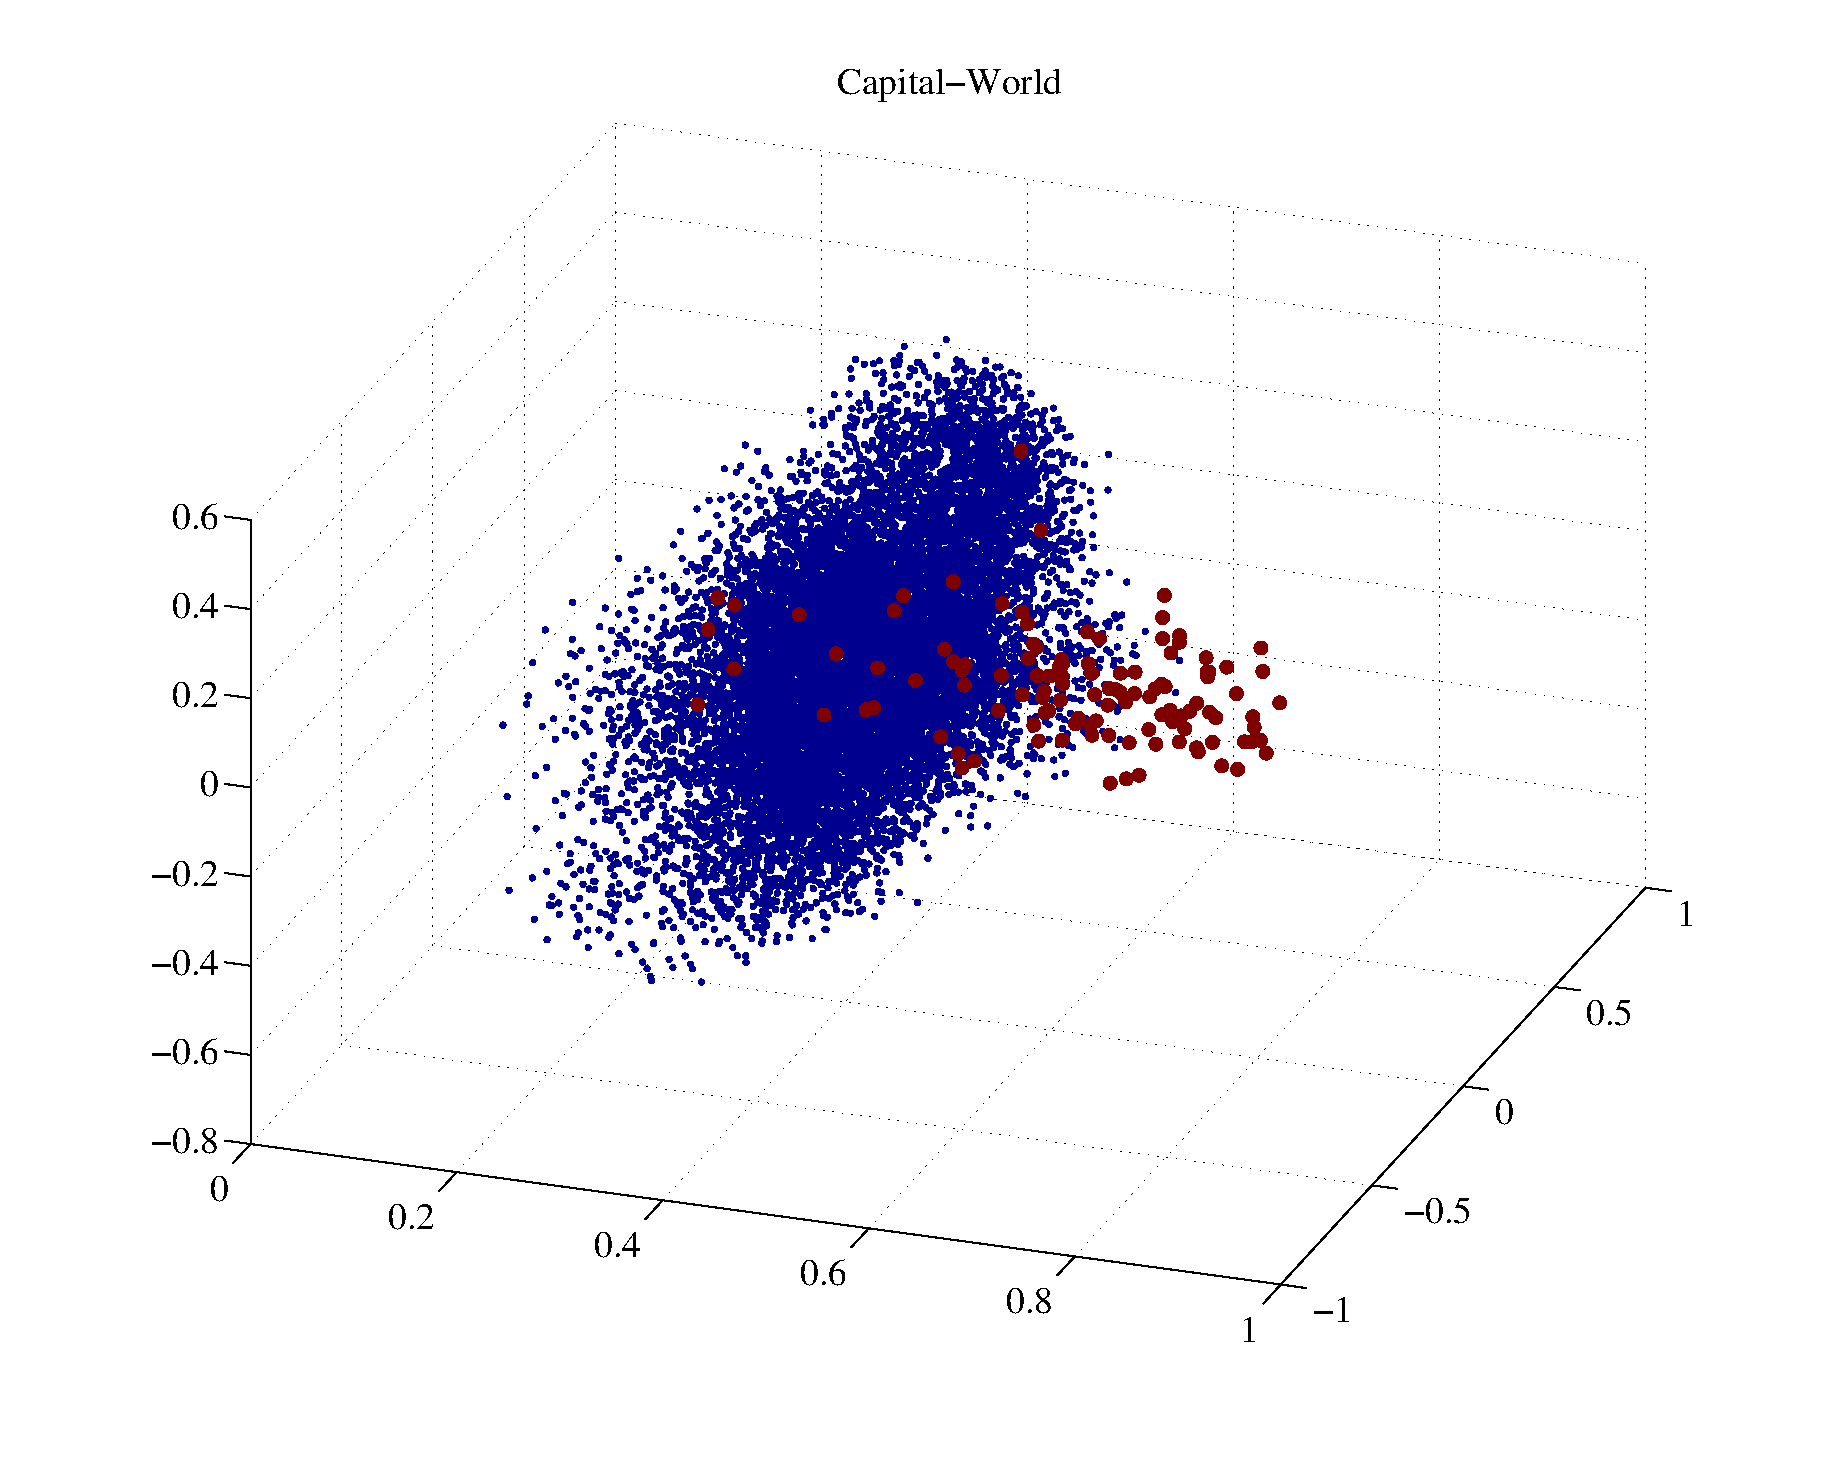
\includegraphics[width=.45\textwidth]{./images/capital_world.eps}
}
\subfigure[Nationality-Adjective]{
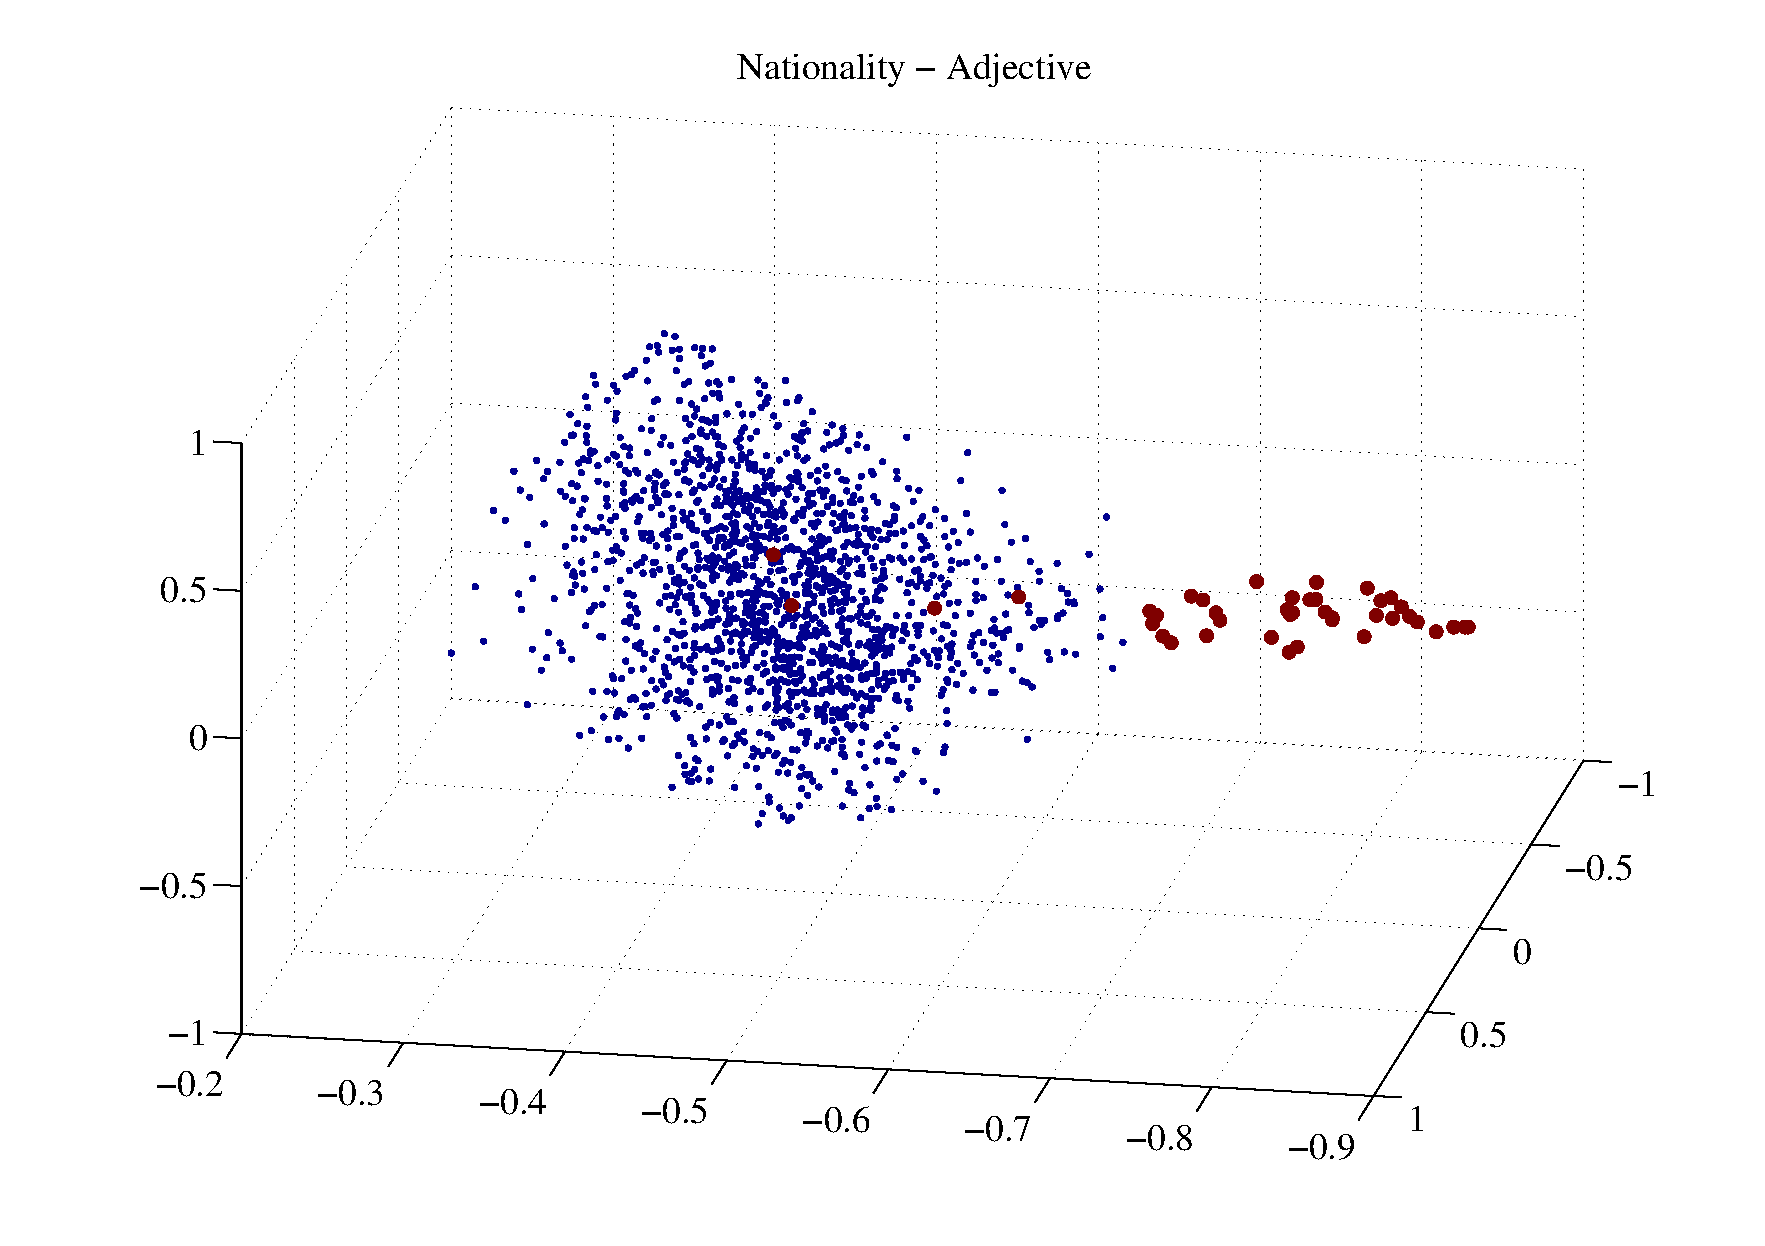
\includegraphics[width=.45\textwidth]{./images/nationality_adj.eps}
}

\subfigure[Plural-Vebs]{
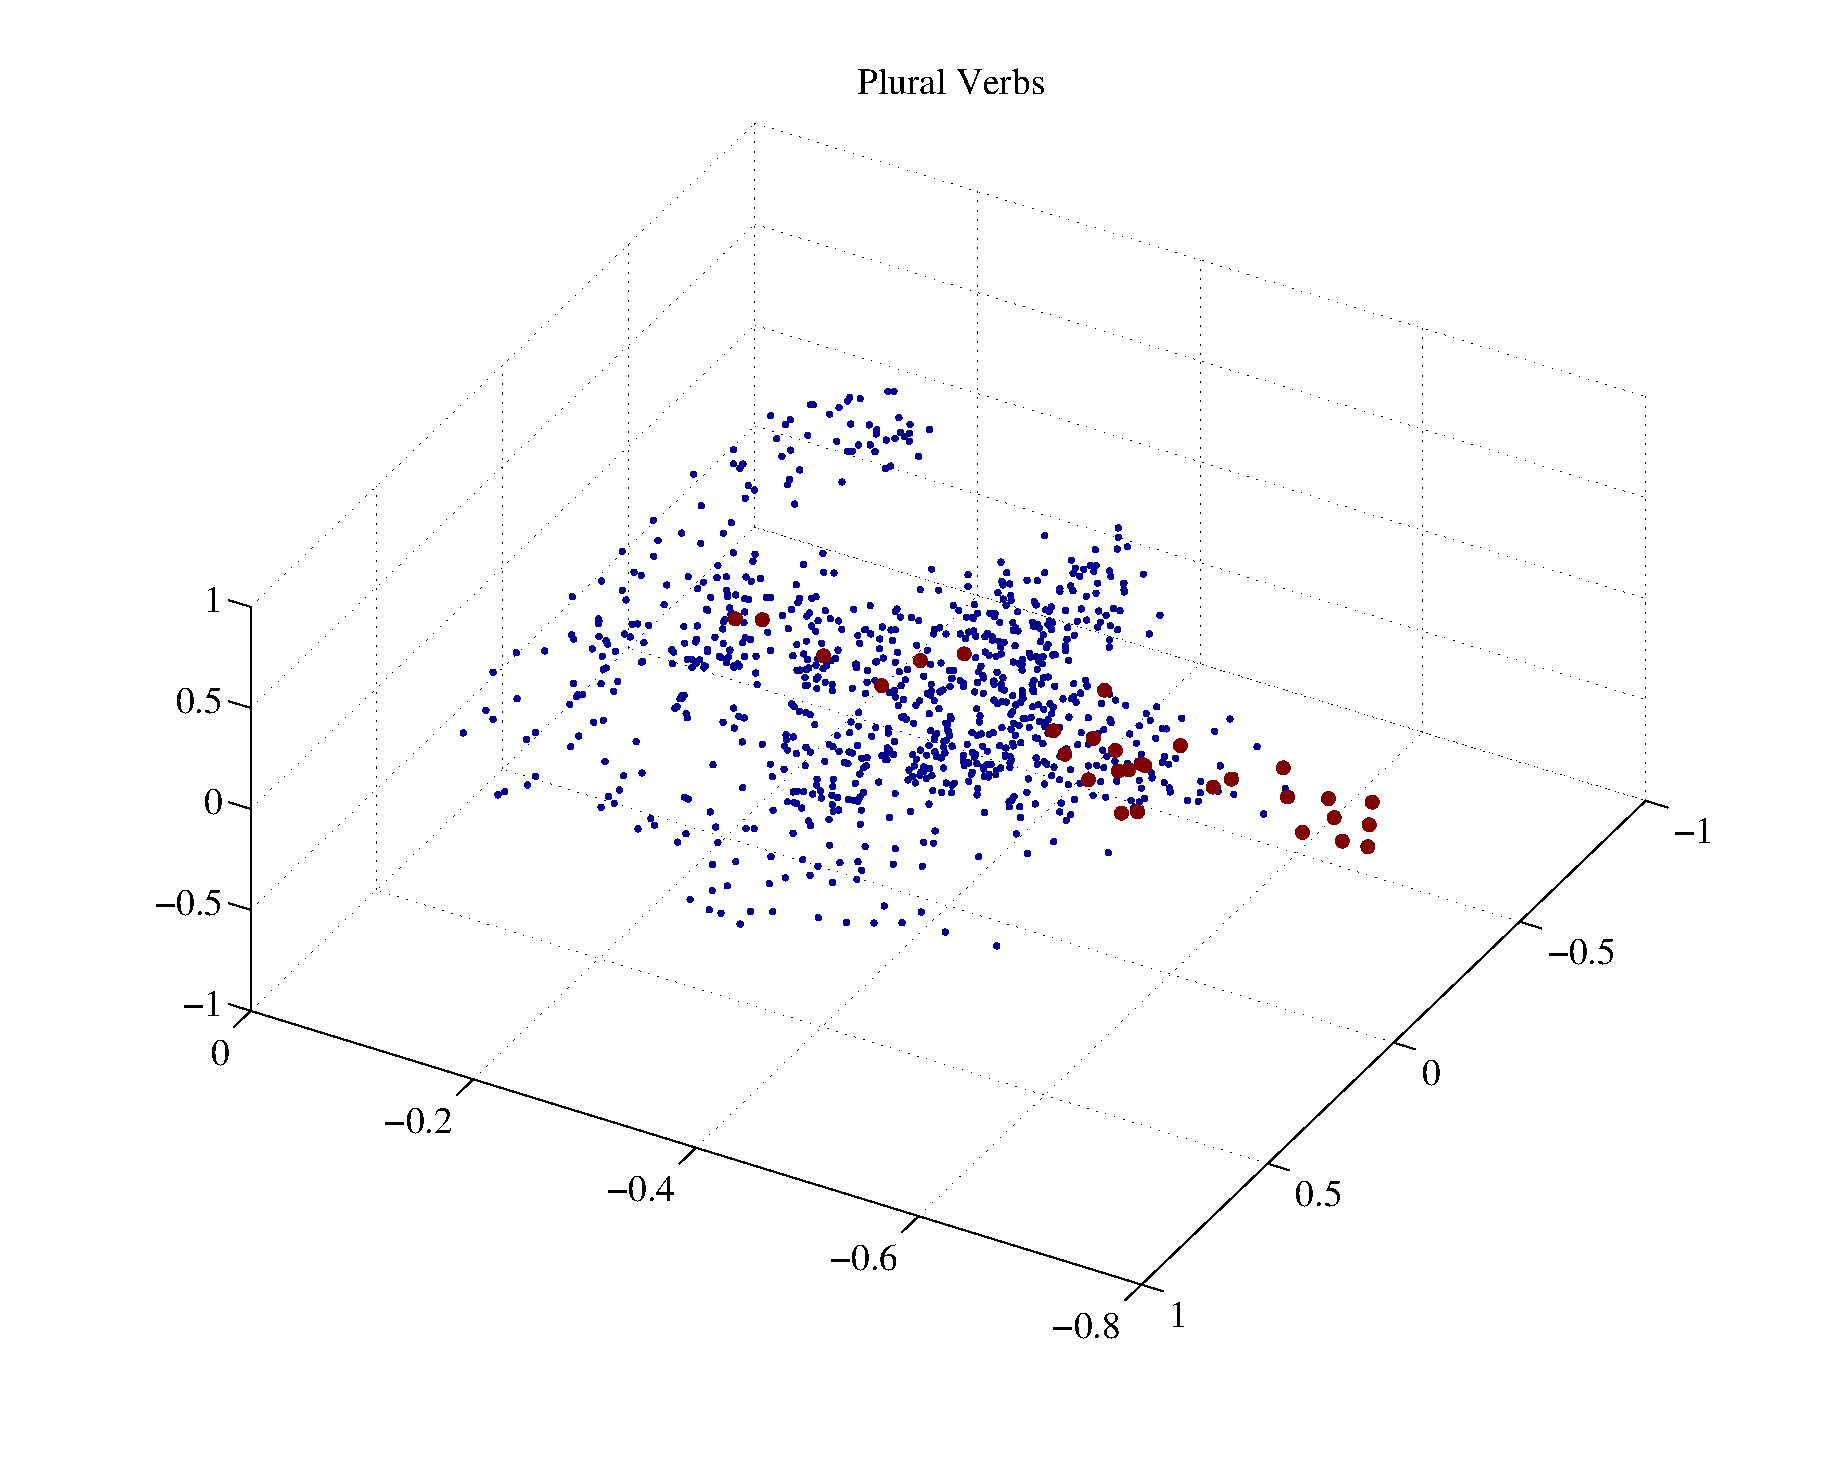
\includegraphics[width=.45\textwidth]{./images/plural_verbs.eps}
}
\caption{Projections of Vector Offsets for different categories of Word-Pairs}
\label{fig:offsetProj}
\end{figure}

\subsection{Low rank approximations of word vectors}
Ideally, we would like to be able to fit a variety of subspaces to all the word vectors. However, in practice the number of word vectors in our embedding space may be too large to afford running a subspace clustering algorithm on the entire set. To with this problem, we generate sets of words related by a high level concept and explore how well the word vectors associated with the set is approximated by a rank $k$ subspace, for varying $k$. If the set of vectors is well approximated by a rank $k$ subspace, for $k$ smaller than the original dimension of the space, then we can conclude the set of word vectors does in fact have linear low dimensional structure. Figure \ref{fig:svdOnClass} shows rank versus the $L2$ approximation error for word vectors in a variety of classes. As the figure shows, some classes are much more amenable to low rank approximations than others. This may partially be a product of our method generating related words (currently being done via a search of the WordNet hierarchy). 


\begin{figure}[t]
\centering
\includegraphics[width=.65\textwidth]{./images/svd_per_class.eps}
\caption{Rank vs. $L2$ error for different sets of word vectors}
\label{fig:svdOnClass}
\end{figure}

\nocite{*}
\bibliographystyle{splncs}
\bibliography{bibliography}

\end{document}
